\documentclass[tikz,border=10pt]{standalone}
\usepackage{tikz}
\usetikzlibrary{calc}
\begin{document}
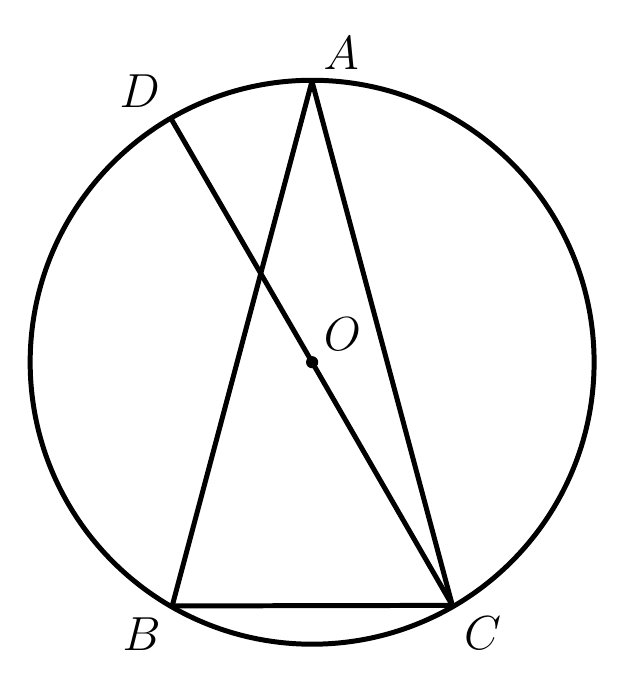
\begin{tikzpicture}[line width=1.8pt, line join=round]
\coordinate (A) at (-0.023,3.348);
\coordinate (B) at (-1.798,-3.315);
\coordinate (C) at (1.760,-3.308);
\coordinate (D) at (-1.807,2.864);
\coordinate (O) at (-0.021,-0.220);



\draw (O) circle[radius=3.581cm];

\draw (A) -- (B);
\draw (A) -- (C);
\draw (B) -- (C);

\draw (D) -- (O) -- (C);

\fill (O) circle (2.200pt);

\node[above right, font=\fontsize{19}{22.8}\selectfont] at (A) {$A$};
\node[below left, font=\fontsize{19}{22.8}\selectfont] at (B) {$B$};
\node[below right, font=\fontsize{19}{22.8}\selectfont] at (C) {$C$};
\node[above left, font=\fontsize{19}{22.8}\selectfont] at (D) {$D$};
\node[above right, font=\fontsize{19}{22.8}\selectfont] at (O) {$O$};
\end{tikzpicture}
\end{document}